\documentclass[12pt]{article}
\usepackage[danish]{babel}
\usepackage{graphicx}
\usepackage[pdftitle={Sorterings algoritmer},pdfauthor={Jens Tinggaard}, hidelinks]{hyperref}
\usepackage{minted}
\usepackage{amsfonts}




\date{\today}
\title{Sorterings algoritmer}
\author{Jens Tinggaard}



\begin{document}
    \maketitle
    \definecolor{bg}{rgb}{0.95,0.95,0.95}

    {\large\tableofcontents}
    \newpage



    \section{Sorterings algoritmer}
    Sortingsalgoritmer er algoritmer som bruges til at sortere lister, eller andre sorterbare ting.
    Der findes et utal af dem, og de varierer i hastighed, hukommelseskrav og fordele/ulemper afhængig af "blandbarheden" af listen.

    En sorteringsalgoritme er kendetegnet ved at den tager en liste $A$ som input, og returnerer den sorterede liste. Længden af en liste er vist som $n$, og index kaldes på  følgende måde: $A_n$, hvilket vil være det sidste element i listen.


        \subsection{Bubble sort}
        \label{sub:bubblesort}
        Bubble sort er nok den mest simple sorteringsalgoritme der findes.
        Den virker ved at sammenligne element $A_0$ med $A_1$ og bytter så elementerne om, i tilfælde af at $A_1$ er større end $A_0$.
        Algoritmen kører hele listen igennem, hvorefter man ved at $A_n$ er sorteret.
        Algoritmen starter så forfra, fra $A_0 \to A_{n-1}$ hvorefter $A_{n-1} \to A_n$ er sorteret.\\
        Det vil sige at algortitmen kører listen igennem $n$ gange i alt.
        Algoritmen har en worst-case på $O(n^2)$ og et gennemsnit på $O(n^2)$. Dog er best-case på $O(n)$ i tilfælde af at listen allerede er sorteret


        \subsection{Insertion sort}
        En anden algoritme, som er forholdsvis ligetil, er insertion sort. Den virker på samme måde som de fleste nok ville sortere kort i hånden.
        Man tager $A_1$ og sammenligner med $A_0$ og bytter om på dem hvis nødvendigt. Nu er $A_0 \to A_{1}$ sorteret.
        Derefter tager man og kigger på $A_2$ og sammenligner med $A_1$, hvis de bliver byttet, sammenligner man også værdien med $A_0$. Og ombytter hvis nødvendigt.
        Nu er $A_0 \to A_2$ sorteret.
        Algoritmen har en worst-case på $O(n^2)$ og et gennemsnit på $O(n^2)$ og ligesom \nameref{sub:bubblesort}, en best-case på $O(n)$.






    \section{Implementering af bubble sort}
    Følgende kodeudtræk er min implementering af bubble sort i Python, funktionen tager, 1 obligatorisk argument, hvilket er listen som skal sorteres: \texttt{A}
    Derudover tager den et boolean, \texttt{show\_progress}, som angiver om listen skal printes for hver ændring af den, sådan at man kan følge og på den måde debugge funktionen.

        \subsection{Bubble sort i Python}
        \begin{minted}[python3, linenos, breaklines, fontsize=\footnotesize, bgcolor=bg]{python}
def bubble_sort(A, show_progress=False):
    """
    Bubble Sort is the simplest sorting algorithm that works by repeatedly
    swapping the adjacent elements if they are in wrong order.
    """

    for i in range(len(A) - 1):
        swapped = False

        for j in range(0, len(A) - i - 1):
            if A[j] > A[j+1]:

                if show_progress:
                    print(A)

                A[j], A[j+1] = A[j+1], A[j]
                swapped = True

        if not swapped:
            break

    if show_progress:
        print(A)

    return A
        \end{minted}
        \label{snip:bubble_sort}
        \begin{center}
            \caption{Kildekode 1: Implementering af \texttt{bubble\_sort()}}}
        \end{center}
        Algoritmen virker som sagt ved at tjekke et givent array \textt{A} igennem, $n$ antal gange. Eller indtil det er sorteret.
        Jeg har bygget det op over et såkaldt "nested" for-loop, hvilket i bund og grund er et for-loop inde i et andet.
        Det yderste for-loop, looper altså over arrayet, $n-1$ gange.
        Mens det inderste looper mellem $n-1$ og $1$ gange - altså det antal usorterede elementer der er tilbage.
        Hvis elementerne ikke er sorteret, bliver de byttet om på, og \texttt{swapped} bliver tildelt værdien $True$.
        Hvis det inderste for-loop når at løbe en hel omgang, uden at bytte om på nogle elementer, vil værdien for \texttt{swapped} være $False$ og det yderste loop bliver brudt, da hele listen nu er sorteret.




    \section{Test af program}
    For at teste mit program, har jeg lavet en fil kaldet \nameref{file:timing}, som udytter biblioteket \emph{matplotlib}\footnote{https://matplotlib.org/users/installing.html}, som er et bibliotek brugt til at plotte grafer og andet statistik.
    Derudover har jeg brugt det indbyggede bibliotek \emph{time}, til at tage tid på de forskellige algoritmer og kunne sammenligne dem.

        \subsection{Korrekthed af program}
        Idet jeg har skrevet de forksellige algoritmer, har jeg selvfølgelig testet at de virker korrekt, dette har jeg gjort ved at give funktionerne et valgfrit argument, kaldet \texttt{show\_progress}, hvilket angiver om listen skal printes for hver gang den ændres.
        Dette har gjort det super nemt for mig at teste korrektheden af hver enkelt algoritme.


        \subsection{Fejlfinding af program}
        Programmet vil formentlig fejle ved:
        \begin{enumerate}
            \item Tomme lister, eller lister bestående af kun 1 element.
            \item Lister bestående af andet end tal (boolske udtryk, tekst strenge osv.)
            \item Andet forkert input $i$ til funktionerne, såsom tal som ikke opfylder $i \in \{\mathbb{N}, 0\}$ for funktionen \texttt{compare()}. Samt at $\emph{upper} \geq \emph{lower}$.
        \end{enumerate}

        \subsection{Eksempel}
        Inden programmet køres, skal det sættes op i \nameref{file:timing}, hvor man angiver antal prøver for hver liste-længde, samt en oppe og nedre grænse for listelængden, angivet i en potens af 10. Syntaksen er som følger:
        \newline
        \begin{minted}[python3, breaklines, fontsize=\footnotesize, bgcolor=bg]{python}
compare(samples, lower, upper, *algorithms)
        \end{minted}
        Kalder man f.eks.
        \begin{minted}[python3, breaklines, fontsize=\footnotesize, bgcolor=bg]{python}
samples = 5
lower = 0
upper = 4

c = compare(samples, lower, upper, merge_sort, tim_sort)
show_comparison(c)
        \end{minted}
        Vil \texttt{merge\_sort} og \texttt{tim\_sort} algoritmerne blive sammenlignet. Med lister i en længde af $10^0, 10^1, 10^3$ og $10^4$. Med $5$ eksempler af hver - listerne er ens for alle de givne funktioner.
        \texttt{show\_comparison()} vil nu plotte resultatet i et nyt vindue som åbner - se figur \nameref{fig:figur1}




        % \begin{figure}
        %     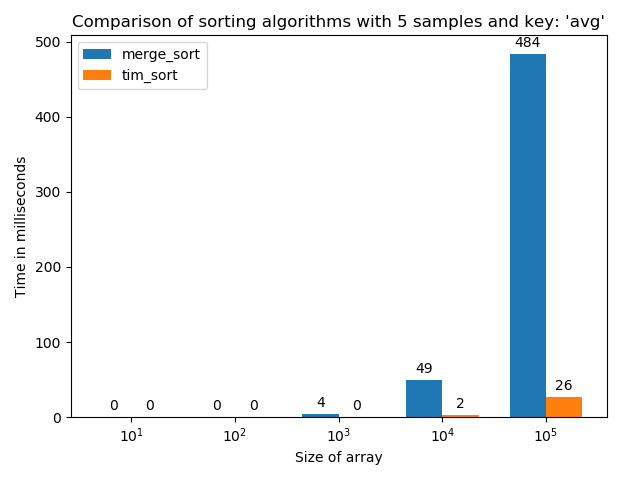
\includegraphics[scale=0.5]{figur1.png}
        %     \caption{Et plot!}
        %     \label{Figur 1}
        % \end{figure}


    \section{Bilag}
    Jeg har uploadet koden til et repo på GitHub, \url{https://git.io/JeEmo}, hent det med git:
    \begin{minted}{bash}
$ git clone https://github.com/Tinggaard/sorting_algorithms.git
    \end{minted}


        \subsection{sorting.py}
        \label{file:sorting}
        \inputminted[python3, linenos, breaklines, frame=lines, fontsize=\footnotesize]{python}{sorting.py}

    \newpage

        \subsection{timings.py}
        \label{file:timing}
        \inputminted[python3, linenos, breaklines, frame=lines, fontsize=\footnotesize]{python}{timings.py}


\end{document}
